% mainfile: ../../../../master.tex
\subsection{Loading ship}
% The part of the label after the colon must match the file name. Otherwise,
% conditional compilation based on task labels does NOT work.
\label{task:20180206_cj0}
\tags{mime}
\authors{cj}
%\files{}
\persons{Mia Cerfonteyn}

We agreed with Mia that it would be easier to organise everything by ourself rather than ordering a taxi. So I used Tómas's car to go pick her up a little after 7:00 AM, then we drove to Matís to load the nitrogen tank and 3 boxes in the car. We drove to the harbour to drop off everything. Mia stayed at the ship to organise the material on the ship as well as her personal belongings while waiting for the liquid nitrogen to be delievered. During this time, I drove back to Matís to pick up the last 2 boxes as well as the big Nalgene platic bottles. When I arrive at the harbour for the second time, the liquid nitrogen arrived just after. We made sure the tank were loaded safely onto the ship, before we finally went back to Matís for lunch.

\begin{figure}[H] % position of the figure 
    \centering
    %\caption{Title of the figure}
    %\label{fig:label}
    \begin{subfigure}[b]{\textwidth}
        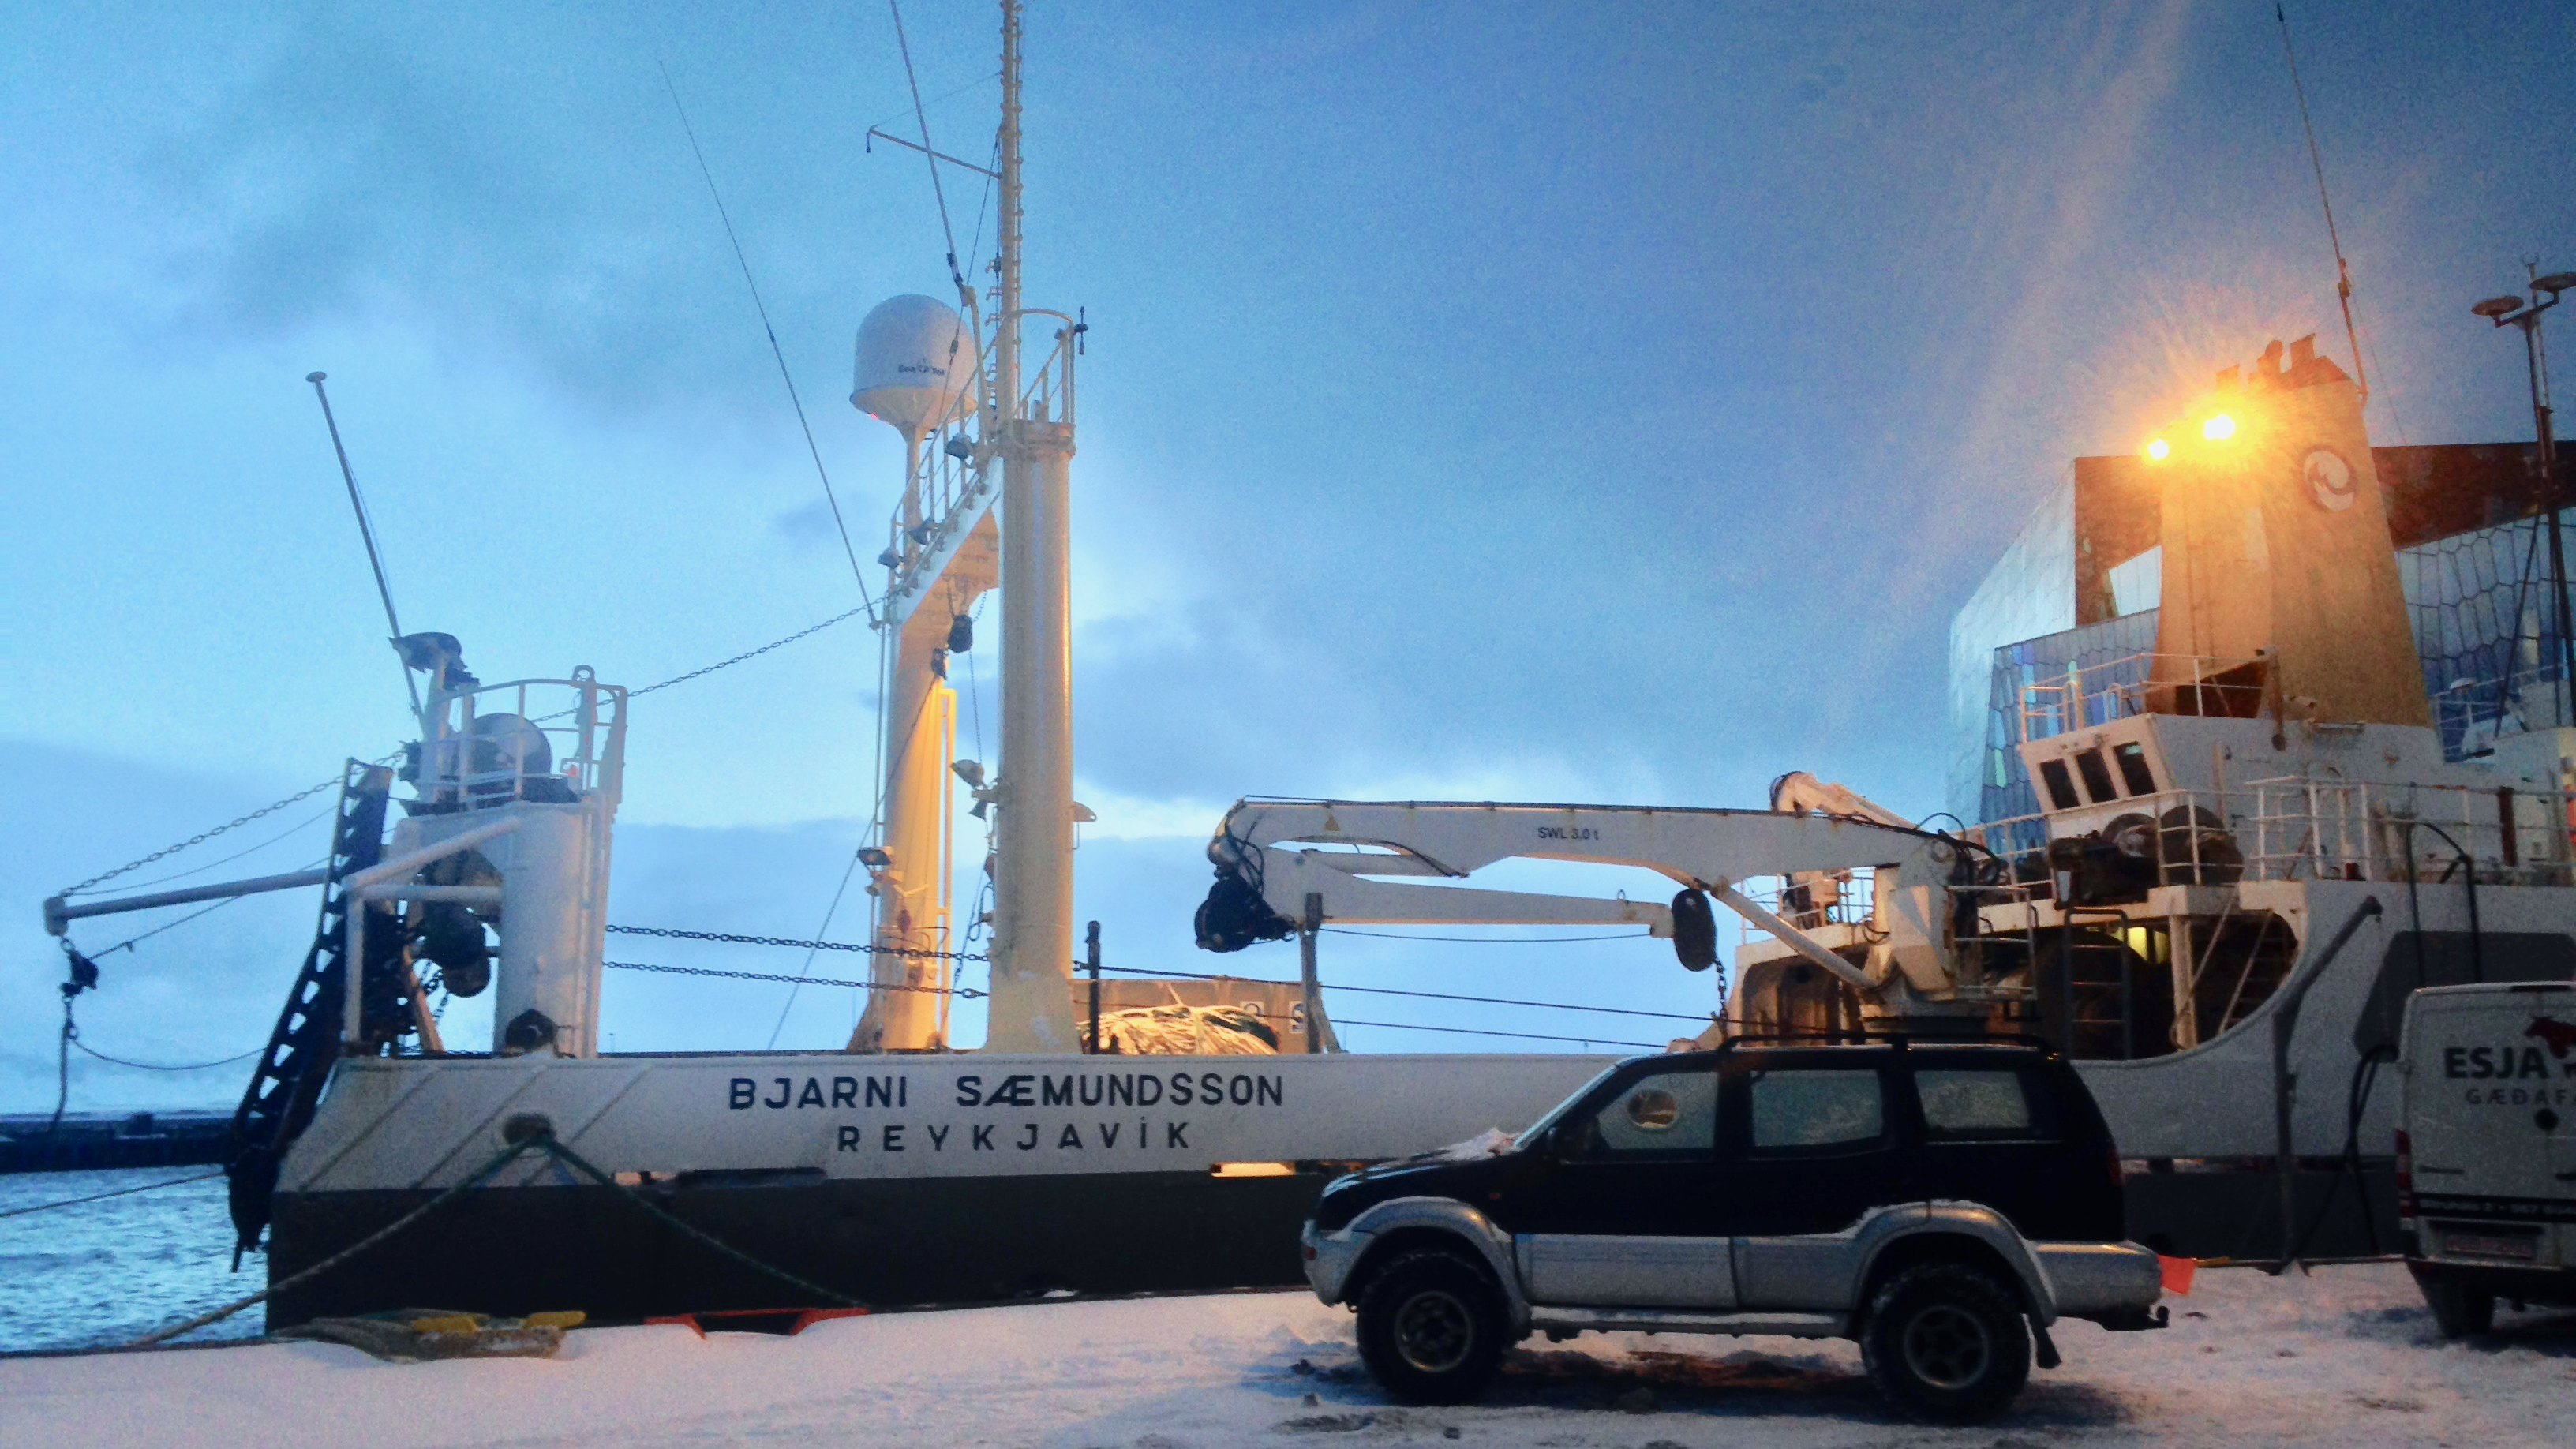
\includegraphics[width=\textwidth]{graphics/pic/20180206_bjarni_saemundsson1.png}
     %   \caption{Bjarni Sæmundsson}
     %   \label{sfig:slabel1}
    \end{subfigure}
    \\
    \begin{subfigure}[b]{\textwidth}
        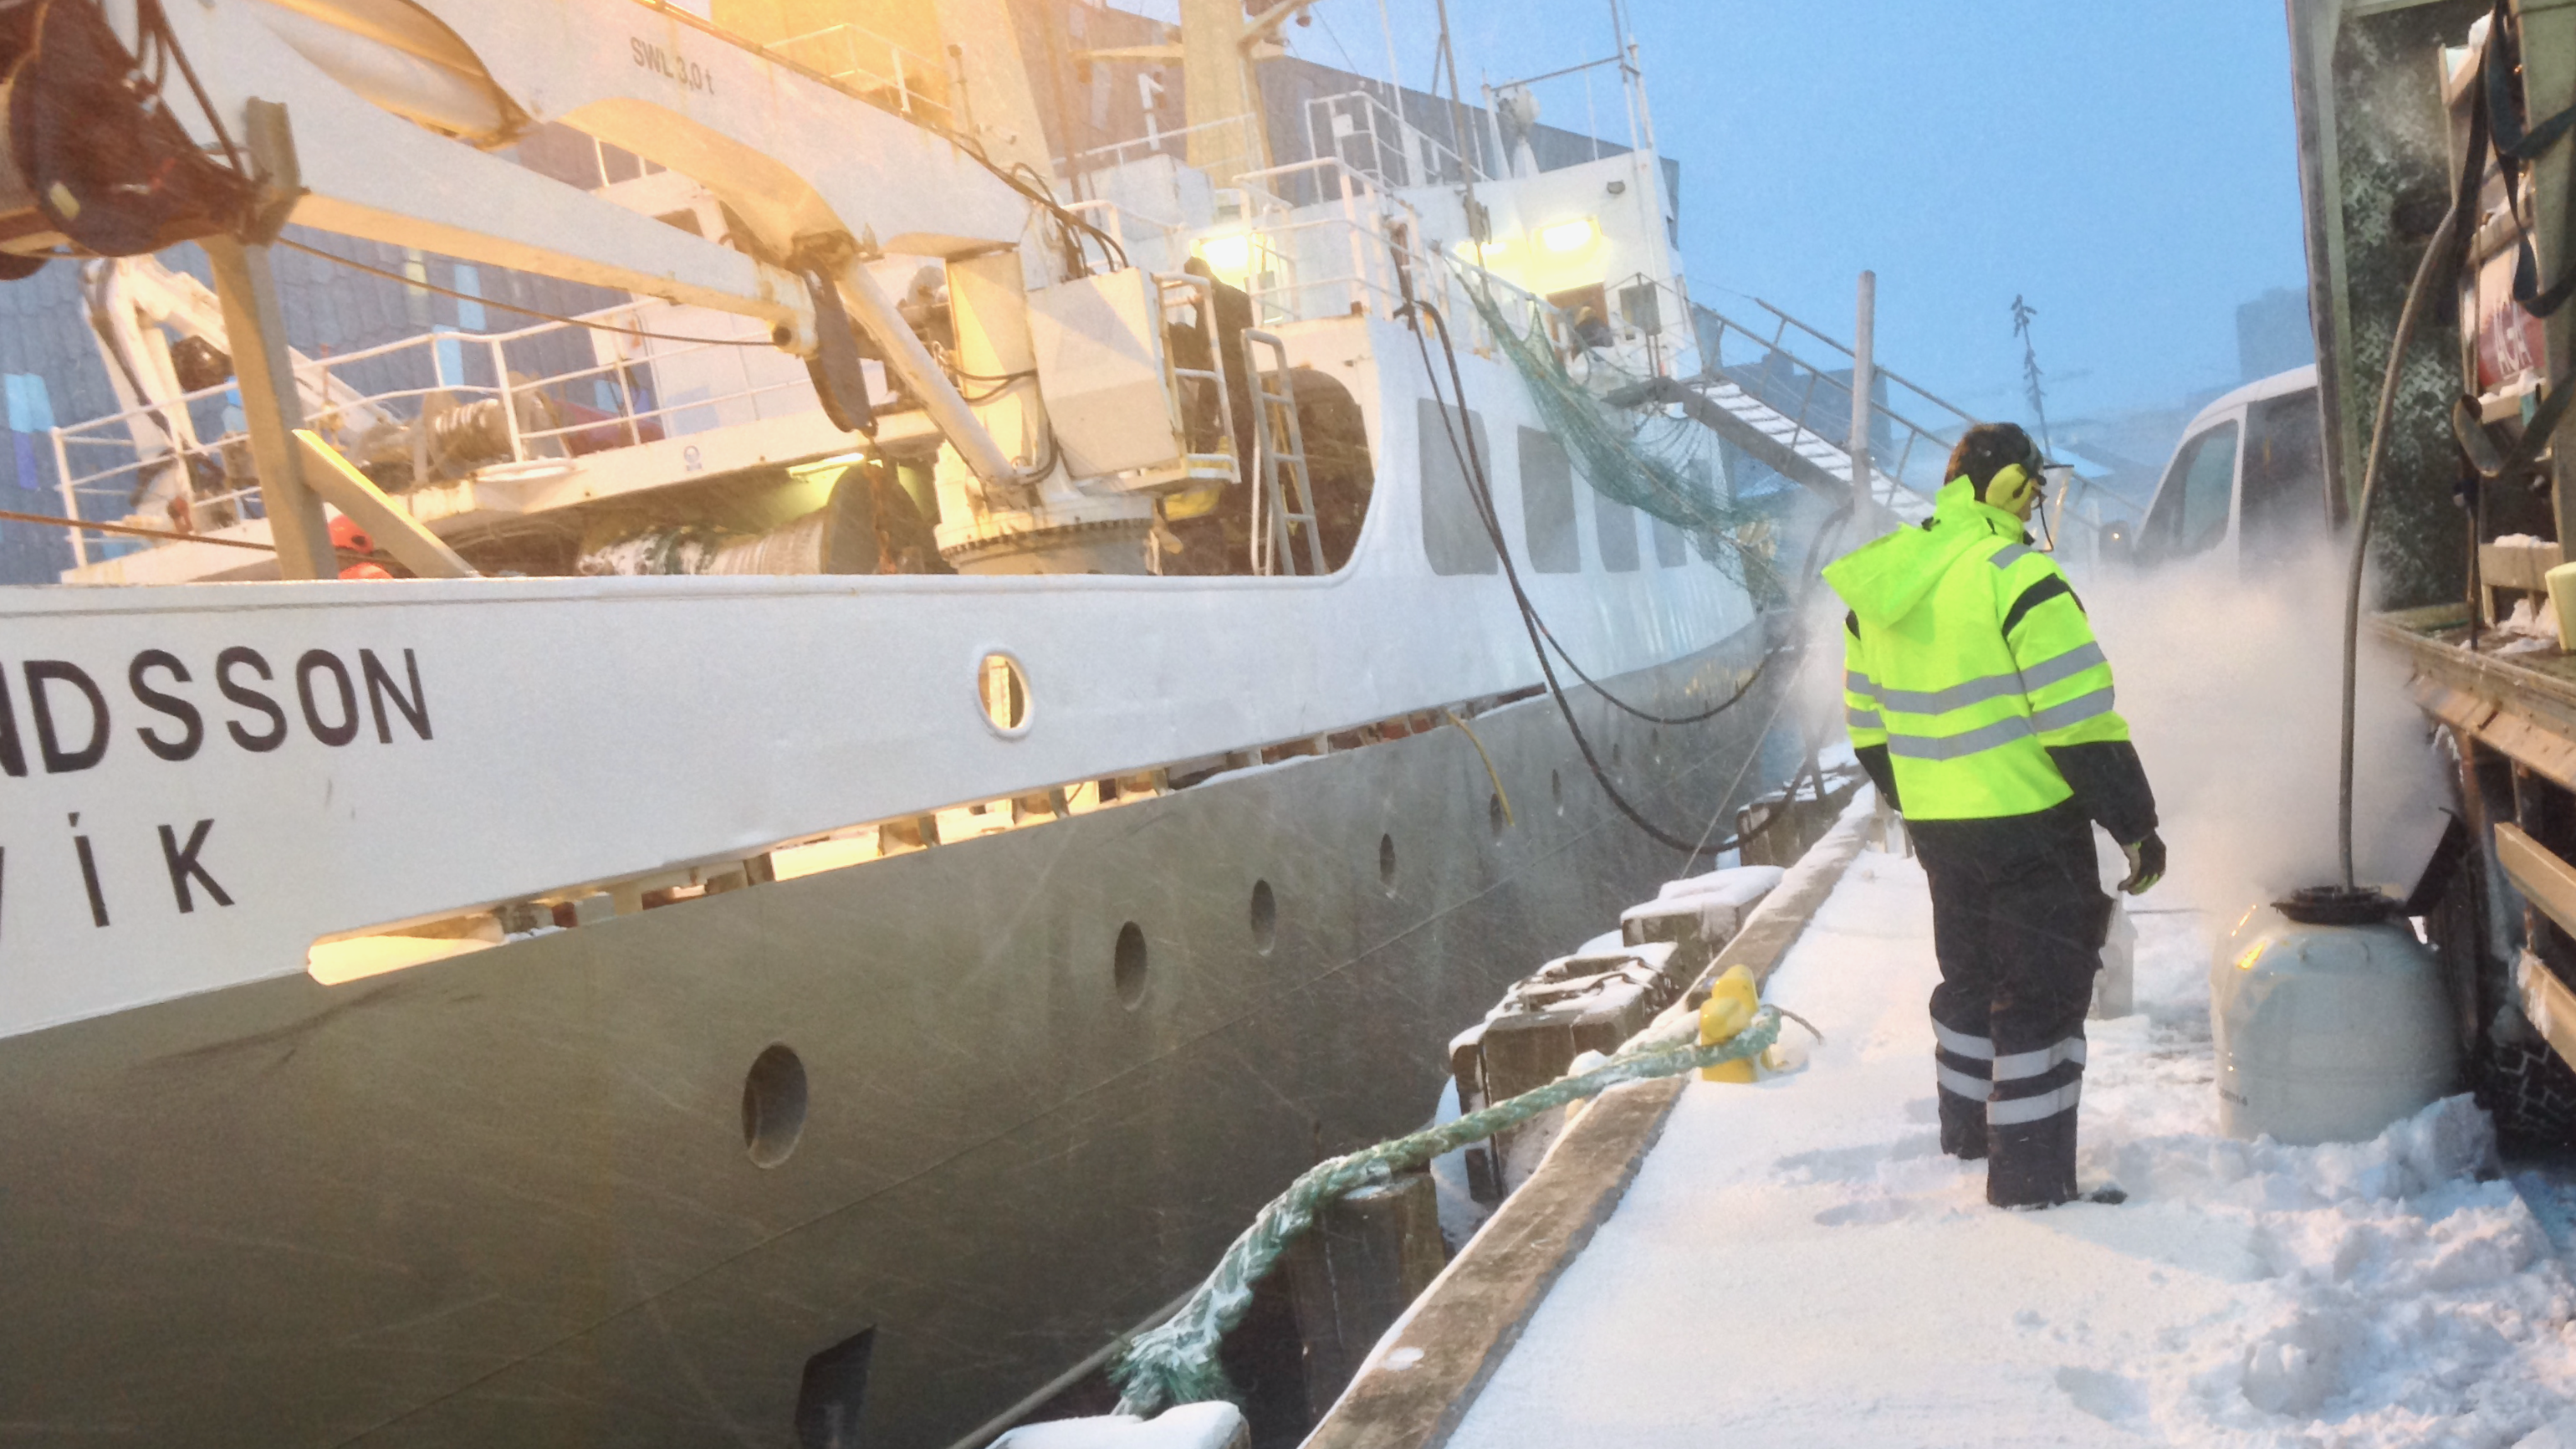
\includegraphics[width=\textwidth]{graphics/pic/20180206_bjarni_nitrogen.png}
      %  \caption{Title of the first subfigure}
       % \label{sfig:slabel2}
    \end{subfigure}
\end{figure}
